%!TEX root = ../crimson_throne_book_main.tex
% 2015-10-10
The companions have seen some strange creatures before, but never have they set their eyes upon a\hyperref[fig:Scrivenite-in-the-vivified-labyrinth-563932189]{ creature made of books and scrolls } . As an avid reader, Quint is amazed and horrified at the same time to face the  {\itshape scrivenite} , unsure of whether attacking it can even be justified. Balian feels no such qualms and bears down heavily on the living documents. Puk finds out that his sneak attacks are once again useless against this being, reducing his roll in the combat to assisting the ranger. At least that is what he was hoping to do, because the scrivenite utters magical words that freeze Balian in place. Fortunately Sjo's quick thinking provides a rapid answer as the Shoanti casts a  {\itshape remove paralysis} to set his friend free again. In return the creature lashes out with its bookmarks. The ribbons do little damage, but they drain some of Sjo's intelligence. Balian sees that the stolen knowledge immediately manifests itself as a new text among the many scrolls on the scrivenite's frame. After that strange occurrence his greatsword and Sjo's fire magic swiftly reduce the enemy to a pile of volumes and parchments again, ending the fight. \\

\begin{figure}[h]
	\centering
	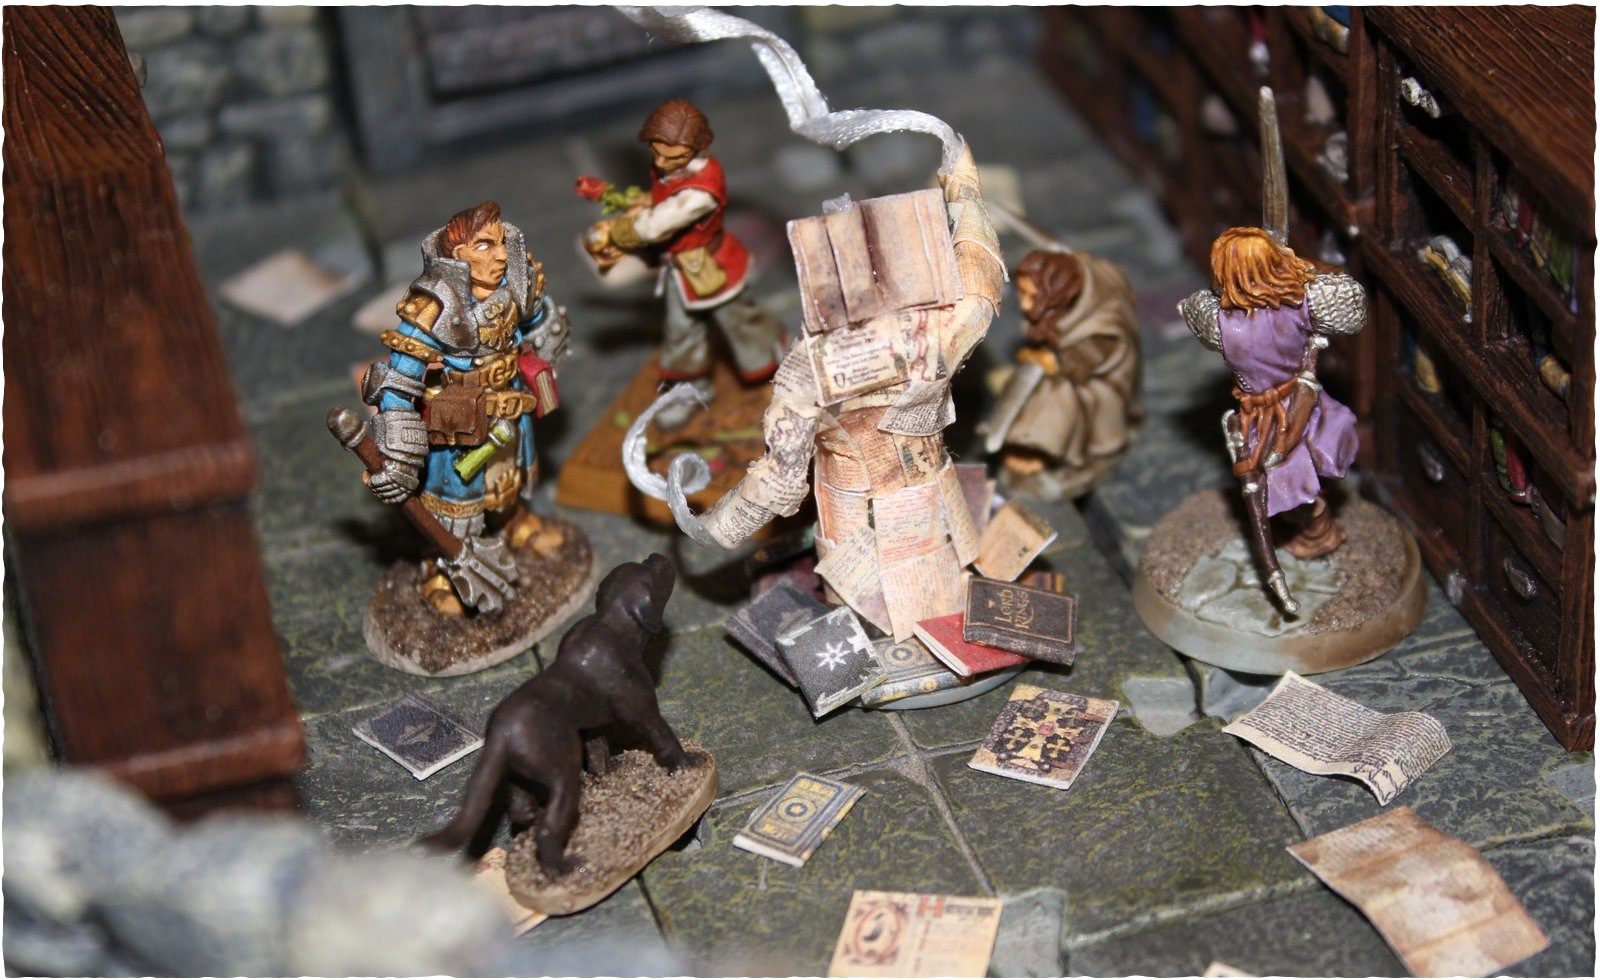
\includegraphics[width=0.4\textwidth]{images/Scrivenite-in-the-vivified-labyrinth-563932189_mod.jpg}
	\caption{Scrivenite in the vivified labyrinth}
	\label{fig:Scrivenite-in-the-vivified-labyrinth-563932189}
\end{figure}

Sjo recovers the text with the memories that were taken from him, but has to hand it to Quint because he does not master the art of reading. As the bard reads the words out loud, Sjo realizes that these recollections must date back to a time that he never consciously remembered. It is the story of his birth, which he can only have learned from the mouth of his mother as a newborn.\\

 {\itshape Yundur Firestorm was his name and he was truly blessed by the power of the sun. His people were the Sklar-Quah, the Sun Clan, the noblest of all Shoanti. After he had finished training as a sun shaman, he was appointed the southernmost tribe of the Sklar-Quah. Yundur was still young and bursting with admiration for his brethren's lust for battle. As their spiritual leader he fanned this flame and enjoyed their hatred for the}  Yes, Yundur Firestorm was truly blessed in his spiritual doings, but he turned out to be equally cursed in his family life. Five times his wife bore a dead son before finally giving birth to a living child, a girl, Aithne (pronounce EFnee). She became the apple of his eye and was trained from a young age to follow in her father's footsteps.\\

But Aithne was more interested in joining the ranks of the famed burn riders than in going through life a boring shamaness. The elite mounted cavalry of the Sklar-Quah, who were able to coax their horses to race through the flames, represented the culmination of Shoanti honor. And so it happened that the disobedient teen Aithne secretly followed the burn riders on a raid in the lowlands. She was joined by her faithful companion Shaoban (pronounce SHEEbuhn), the jothka's son, whom his father, the chief, still deemed too young to go to war.\\

From afar the two youngsters witnessed how the burn riders attacked and burned down some remote farms. When the riders were gone, the curious teens wanted to examine the smoldering field of battle. Shaoban already felt like a warrior and pretended to kill the farmers all over again with his spear. As he proudly jammed his weapon through the skull of a dead farmer's wife, the corpse next to her suddenly arose. His face was red with blood, and even though he was hardly any bigger than Shaoban, he jerked the spear out of the surprised Shoanti's hands and thrust it through his chest. Then he turned on Aithne and knocked her out with the blunt end of the weapon.\\

When the girl woke up, she was naked and smeared with blood and soot. Shaoban's severed head towered above her on a wooden stake. From his eyes protruded two arrows. Just a few yards away the surviving farmer's son was finishing his family's grave. Aithne crawled to her feet and started to flee in utter fear.\\

"Run all you can, barbarian spawn!" a rough voice called out. "Flee to your people and tell them that they will all end up like this wretched creature here! And explain how a whore like you wound up with Chelaxian seed in her belly!"\\

His maddening laughter haunted her across the fields and kept ringing through her head for hours, while she tried to process what had happened. Apart from the blood on her upper body - which clearly came from her attacker - her own blood was dripping between her legs, proving that his vicious words were true. Did she really have a Chelaxian's seed in her body? Then she could not return to her people, not until she was sure that his seed had not taken root.\\

The next couple of weeks the girl roamed the lowland plains and found out that her worst nightmare had come true: she was pregnant with the vengeful farmer's son's child. Her people had never shown understanding or tolerance for bastards and the shame would kill her and her father, so she decided not to head back home before she had got rid of the halfbreed. Killing her own unborn child was no option, as it was the greatest sacrilege imaginable. Therefore she retreated deeper into the lowlands, fleeing every living soul she encountered, until she came upon an abandoned shepherd's hut. There she stayed until her belly was full and she bore a child during a stormy night.\\

The baby was a healthy son, whom the heart-broken mother named for her lost friend, Shaoban. She carved his name in a piece of wood and placed it with the newborn in a wicker basket. With tears in her eyes she begged the sun for help and through her hands flowed a shaman's power which put the child to sleep. Next she entrusted the child's floating cradle to the river, before turning around and commencing the long road home to her tribe.\\

Two days later the basket washed ashore in the city of Korvosa. Shaoban awoke from a long sleep and the starved nursling started crying loud enough to get half the city out of its bed. Some kids who were scavenging the shores of the river's mouth, found the baby and took it home to their cruel master, Gaedran Lamm. And so it was that the young Shaoban wound up with the lambs. Bullheaded Lamm misinterpreted the name on piece of wood and read it as Sjoban, which was later shortened to Sjo.\\

